% -*- root: Document.tex -*-

\section{System components}
\label{sec:sys_components}

From a high-level perspective, \GP is composed of three main components:
\begin{itemize}
  \item The \emph{monitoring} module is responsible for keeping track of resources consumption in the system.
  \item The \emph{placement and migration} module handles the deployment of containers and their relocation to different nodes as they move across generations.
  \item The \emph{scheduling} module contains the algorithms that orchestrate and take decisions regarding container placement and migrations, based on the input received from the monitoring module.
\end{itemize}

The role and interactions between these components are schematically illustrated in Figure~\ref{fig:components}.

\begin{figure}[H]
  \centering
  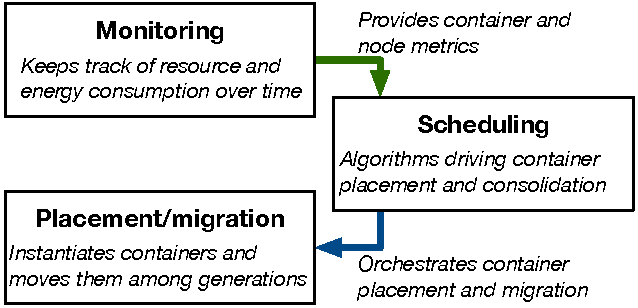
\includegraphics[]{figures/components}
  \caption{\GP's abstract components and their interactions.}
  \label{fig:components}
\end{figure}
